\documentclass{article}
%% \usepackage{amsmath}
\usepackage{amssymb}
\usepackage{algorithm}
\usepackage[noend]{algpseudocode}
%% \usepackage[noend]{algorithmic}
\usepackage{mathtools}

\newcommand{\SA}{\emph{SA} \hspace{1pt}}
\newcommand{\SAT}{{$SA_T$} \hspace{1pt}}

\begin{document}
This writing is about an idea on how to solve the intention progression problem (IPP) with various and complex types of goals and norms. We assume that general notions and concepts in BDI agent and IPP are already known so that the following content can focus on our target problem and the corresponding approach.
\section*{Problem Description}
The problem we want to solve is that when the agent is required to achieve complex of goals and comply complex norms, how should the agent progress (or adopt) its intentions. Here, the meaning of "complex" is related to time and order.
%
Traditionally, a goal specify a certain world state the agent wants to bring about (or maintain if it is a maintenance goal), e.g., visiting a certain place, keeping the floor clean, etc. The goal conditions are usually represented as First-order Logic (FOL) formulas. Although this makes it convenient to implement agent programs, the expression power is limited. In practical applications there may be goals that cannot be captured by basic achievement or maintenance goals. For example, in a Mars rover scenario, the rover agent may have a (complex) goal to collect materials in a certain place and carefully transport them back to a depot. This task is not captured by an achievement or maintenance goal. Rather, it is better modelled by a combination of achievement and maintenance goals: the agent first tries to visit the specified place for collecting materials (achievement goal), then try to go back to depot (achievement goal); during the time when the agent is transporting, it must maintain its speed below a certain level in order to prevent the materials from being damaged (maintenance goal). In practical BDI agent programming languages and platforms, it is hard to design a plan for such complex goals. It is usually the case that complex goals are separated into multiple basic goals and their related plans is separately designed or generated.

%
Although it is possible to directly implement a complex goal using combination of basic goals, encoding the rules and order in these goals is hard, especially when the complex goal is really complex. Dastani\cite{DBLP:conf/atal/DastaniRW11} proposed a uniformed approach to represent complex goals using linear temporal logic (LTL) formulas (they call temporal goals) and described a mechanism for translating temporal goals to basic goals for practical usage considerations. However, their mechanism is hard-coded, only provides transformation rules for common forms of LTL formula; other forms of LTL formula require the user to manually handle. Besides, they only consider the translation from LTL formulas to basic goals, the problems about what plans to adopt and how to interleave multiple intentions are not considered. Although it is possible to separate the concern of LTL translation and the scheduling of the active intentions, it may cause the scheduler to lose the information about how the LTL formulas can be satisfied and consequently trapped in local optima.

%
The idea of using LTL to represent complex goals also apply to norms.
We argue that the scheduler should take LTL formulas as input objects and decides what basic goals and norms should be adopted, what plans to execute and how to execute them to satisfy these LTL formulas (we assume that a plan library is already provided).

\section{Representation and Method}
Here we first define the environment and its state transitions. Based on which, we can give the formal representation of complex goals and norms using LTL.

\subsection*{Environment}
Gutierrez et al.\cite{DBLP:conf/time/0001KPW22} described a model to represent environment and its state transitions. Here, based on their work, we represent an environment as follows.

We assume that the agent acts in an environment that can be in any state of a set $\mathcal{S}$ containing all possible environment states\footnote{We assume that each environment state is identified by a set of ground (first-order) atomic formulas that describe the environment.}. The environment starts from state $s_0$. The agent has a set of actions $\mathcal{A}$. The actions in $\mathcal{A}$ can be performed when their preconditions are satisfied. The postconditions of an action $a \in \mathcal{A}$ in a state $s \in \mathcal{S}$ is transforming $s$ into another state $s^\prime$. This is determined by a transformer function $\mathcal{T} (s, a) = s^\prime$ (we assume that the transformation is deterministic). Here, we focus on the environment state and its transitions. The agent itself and its internal states are not included in the following representation, only the agent's actions that directly affect the environment states are considered.

Formally, an environment is defined by a structure $E=(\mathcal{S}, \mathcal{A},\mathcal{T}, s_0)$ where:
\begin{itemize}
    \item $\mathcal{S}$ is a non-empty finite set of states containing all possible environment states.
    \item $\mathcal{A}$ is the set of actions that the agent can perform.
    \item $\mathcal{T}: \mathcal{S} \times \mathcal{A} \rightarrow 2^{\mathcal{S}}$ is the transformer function.
    \item $s_0 \in \mathcal{S}$ is the initial state of the environment.
\end{itemize}

An agent follows its strategy to execute actions until there is no action executable or all its goals are achieved. In this way, the action executions in an environment traces out an interleaved sequence of environment states and actions. We call this sequence a \emph{run}:
$$\rho=s_0 \xrightarrow{\text{$a_0$}} s_1 \xrightarrow{\text{$a_1$}} s_2 \xrightarrow{\text{$a_2$}} \cdots \xrightarrow{\text{$a_{n-1}$}} s_n$$

Where $\rho$ is a run, we use $si(\rho, u)$ to index the $u$th state and $ai(\rho, u)$ to index the $u$th action in $\rho$ ($u$ is a natural number). We assume a run $\rho$ is finite, i.e., there is a final state $s_n$ representing the end of $\rho$.

\subsection*{LTL Representation}
LTL is a modal temporal logic with modalities referring to time. In order to represent complex goals and norms by LTL (we call LTL object), in addition to conventional propositional logic operators we consider 3 tense operators: $\square$ ("always..."), $\Diamond$ ("eventually...") and $\mathsf{U}$ ("...until...").

Each LTL object delivered to the agent corresponds to a basic goal or an organized combination of basic goals. We assume that the user gives information about what reward the agent can get if The LTL is satisfied. The following are some expamles on the relationship between LTL objects and basic goals or norms.

%
An LTL object $\Diamond s_g$ corresponds to an achievement goal for reaching a world state $s_g$. This means that the agent is required to bring about $s_g$ eventually at some point in time.
%
$\square s_m$ corresponds to a maintenance goal for always maintaining $s_m$.
%
$\square (\tau \rightarrow ( \Diamond done(a) \mathsf{U} \mu))$ corresponds to a prohibition norm where $\tau$ is the activation condition and $\mu$ is the deactivation condition, $done(a)$ denotes the fact that action $a$ is performed. The triggering condition means that after $\tau$ is satisfied, performing action $a$ before $\mu$ is satisfied triggers the norm and will receive value of $Val$. $Val$ can be positive or negative indicating either an obligation norm (the agent is required to perform $a$) or a prohibition norm (the agent is prohibited to perform $a$). We assume that the norms are implemented as soft constraints, thus not limiting the agent's flexibility. The agent can choose obeying or violating the norm accordingly with respect to the value $Val$ and its own strategy.

The complex goal example mentioned in the previous section can be represented by LTL as:
$$\Diamond c \land (\Diamond c \rightarrow \Diamond t) \land \square (c \rightarrow (s{U} t))$$
where, $c$ is collecting materials, $t$ is transporting materials back to depot and $s$ is slowing down the speed. This means that the agent is required to first adopt an achievement goal to collect materials ($c$); once it is achieved, the agent needs to adopt another achievement goal to transport the materials back to depot ($\Diamond c \rightarrow \Diamond t$); during the period of transporting, the agent needs to keep its speed slow ($\square (c \rightarrow (s{U} t))$).

\subsection*{Our Approach}
% MCTS
The state-of-the-art approaches to IPP is \SA which is based on Monte-Carlo Tree Search (MCTS). However, \SA only considers achievement goals; in the simulation phase of \SA, the total value obtained for achieving goals is returned at the end of every simulation run. Because the goal condition is defined as a set of propositional literals, the checking process is rather strait straightforward: if the goal condition is satisfied, the goal is achieved. However, when LTL goals and norms (we call LTL objects) are included, we need extra algorithms to check whether a given LTL formula is satisfied.

% LTL --> automata
\subsection*{LTL checker}
In order to support intention scheduling with LTL objects, we first need a mechanism to check whether a run (or partial run) satisfies a given LTL formula.
%
Here, we describe a basic framework to check whether an LTL is satisfied in a given run $\rho$ (a sequence of state transitions).

The basic framework of the LTL checker are shown in figure \ref{fig:checker}.
\begin{figure}[h!]
    \centering
    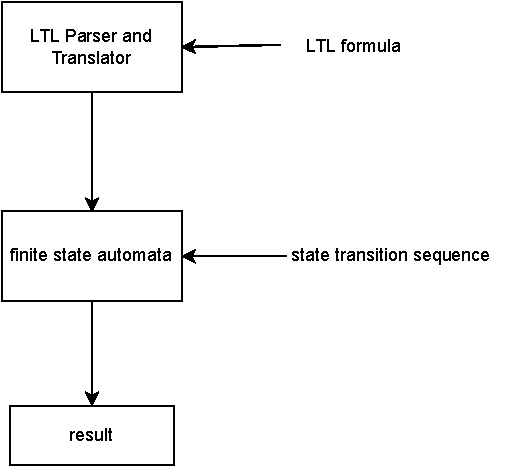
\includegraphics[scale=0.5]{translator.pdf}
    \caption{LTL checker}
    \label{fig:checker}
\end{figure}
The checker first uses LTL Parser and translator to translate an LTL formula to its equivalent automaton, then the state transition sequence is checked by the automaton.

The LTL parser and translator are already implemented in \cite{DBLP:books/daglib/0020982} and \cite{DBLP:journals/jlap/HuangC22}.
% finite and infinite
In \cite{DBLP:books/daglib/0020982}, the automata are specifically for checking infinite state sequences while in \cite{DBLP:journals/jlap/HuangC22}, the automata are for checking finite state sequences.

% note
This checker can be used to check any types of LTL objects. If multiple LTL objects need to be checked, two options are available. One is to process each LTL formula at a time and the other is to use conjunction to represent multiple formulas as one formula and then be processed by the checker.

The algorithm for checking a LTL object $o$ in a run $\rho$ is shown in algorithm \ref{checker}.
\begin{algorithm}
\caption{LTL Checker}\label{checker}
\begin{algorithmic}[1]
\Procedure{Check($\rho, o$)}{}
\State $l \gets getLTLformula(o)$
\State $\alpha \gets translate(l)$ \Comment{translate the LTL to an automaton}
\For{$i \leftarrow 0, len(\rho)-1$}
\State $s \gets si(\rho, i)$
\If {$\alpha.isTransitable(s)$}
\State $\alpha.transit(s)$
\Else
\State \Return $false$
\EndIf
\EndFor
\If {$\alpha$ is in its final state}
\State \Return $true$
\Else
\State \Return $false$
\EndIf
\EndProcedure
\end{algorithmic}
\end{algorithm}
The checker takes 2 parameters as input: a run $\rho$ and a LTL object.
%
The checker first gets the LTL formula and transform it into an automaton (line 2-3). Then, each state in $\rho$ is iteratively processed by the automaton (line 4-9): if the automaton is transitable in the current checking state, the transition is applied. Otherwise, the automaton doesn't accept current state. After $l$ is processed, the checker then checks whether the automaton is in the final accept state, and return the corresponding result (line 10-13).

Here, we describe the mechanism of how to adopt basic goals based on given LTL formulas.
% initial setup
Assuming that an agent is initially allocated with a set of LTL objects; before its execution, the agent first transforms each of the LTL formula into an automaton (automata are encoded as a part of the agent's internal state). 
% execution
When the agent is in execution, each time the agent's belief base is updated, all automata are updated (state transition applied) according to the agent's current beliefs and basic goals or norms are adopted according to the current state of each automaton. For each automaton, there is a path from current state to the final accept state, the agent needs to decide which basic goal or norm should be adopted in order to reach the final state. If there is no transition rule to be applied for the current state in an automaton, the automaton doesn't change.

Figure \ref{fig:auto} illustrate the process of the state transitions in an automaton and the resulting basic goal adoption (for the purpose of exemplification, we ignore the failure state). The automaton is translated from the previous complex goal example $\Diamond c \land (\Diamond c \rightarrow \Diamond t) \land \square (c \rightarrow (s{U} t))$ where, $c$ is collecting materials, $t$ is transporting materials back to depot and $s$ is slowing down the speed. This complex goal states that the agent first needs to visit the specified place for collecting materials, then try to transport the materials to the depot; during the time when the agent is transporting, it must maintain its speed below a certain level in order to prevent the materials from being damaged. Initially, the agent is in state $q_1$, in order to follow the path to final accept state, the agent first try to reach state $q_2$ by adopting an achievement goal to satisfy $c$ (materials collected), after $c$ is achieved, the current state is changed to be $q_2$. In $q_2$ there is an arrow pointing towards itself, the agent adopts a maintenance goal for maintaining $s$ (keep the speed slow); the agent also adopts an achievement goal to satisfy $t$ (materials transported) for reaching the final accept state. After $t$ is satisfied, the automaton is in the final accept state, indicating that the complex goal is achieved.
\begin{figure}[H]
    \centering
    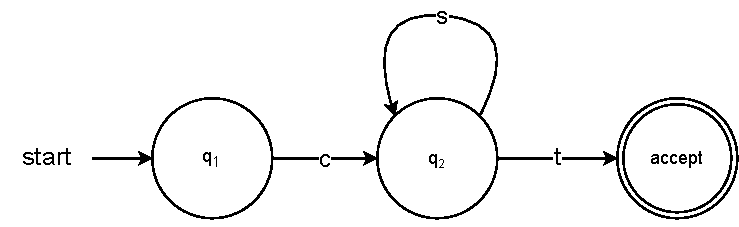
\includegraphics[scale=0.8]{auto_example.pdf}
    \caption{An example of the automaton}
    \label{fig:auto}
\end{figure}

\subsection*{Algorithm}
To support intention scheduling with LTL objects we modify the expansion and simulation phase of \SA.
While norms are not considered in the following algorithms, incorporating them is straightforward.
\begin{algorithm}[H]
\caption{Expansion}\label{mg_expand}
\begin{algorithmic}[1]
\State input:$(n_s)$
      \State $N \gets \emptyset$
      \State $s \gets getWorldState(n_s)$
      \State $AT \gets getAutomata(n_s)$
      \State $I \gets getIntentions(n_s)$
      \For{each $auto \in AT$}
        \State $cas \gets auto.currentState()$
        \For {each $nas \in auto.nextStates()$}
          \State $ws \gets targetWorldState(cas, nas)$
          \If{a basic goal for achieving or maintaining $ws$ is already adopted}
            \State $continue$
          \EndIf
          \If{$nas == cas$}
            \State adopt a maintenance goal for maintaining $ws$ and update $I$
          \Else
            \State adopt an achievement for achieving $ws$ and update $I$
          \EndIf
        \EndFor
      \EndFor
    \For {each $i \in I$}
      \State $Act \gets getExecutableActions(i)$
      \For{each $a \in Act$}
        \State{$i.progress(a)$}
        \State $s_e \gets s.apply(a)$
        \For{each $auto \in AT$}
          \If{$auto.isTransitable(s_e)$}
            \State $auto.transit(s_e)$
          \EndIf
        \EndFor
        \State $n \gets newNode(s_e, AT, I)$
        \State $N \gets N \cup \{n\}$
      \EndFor
    \EndFor
    \State $n_s.setChildren(N)$
    \For{each $n_i \in N$}
    \State $n_i.setParent(n_s)$
    \EndFor
\end{algorithmic}
\end{algorithm}

\paragraph{Modifications to the expansion phase}
In the expansion phase, a selected leaf node $n_s$ is expanded according to the agent's current executable actions. Before checking executable actions in each intention, the agent needs to determine what new basic goals should be adopted according to current automaton (line 6-15): for each automaton, the agent first identifies current state of the automaton $cas$, then check each possible next state $nas$ and (by calling the function $targetWorldState(...)$) get the target world state\footnote{Automata state and world state are different, how an automaton transit its state is determined by the world state and not the other way around.} $ws$, \textbf{which the agent needs to satisfy in order to transit from $cas$ to $nas$} (line 7-9). Whether to adopt a new basic goal and what basic goal to adopt are determined by the relationship of $cas$ and $nas$ (line 10-15).
%
Next, the agent checks each of its intention $i \in I$, progress $i$ according to each of the executable actions $a \in Act$ in $i$. The postconditions of $a$ are applied on $s$ to get the resulting world state $s_e$, and $s_e$ is used to update each automaton $auto \in AT$ (line 20-23). Then, each new node is generated according to the updated $s_e$, $AT$ and $I$(line 24). Finally, all new nodes are set as the children of $n_s$ (line 26-28).

\begin{algorithm}[H]
\caption{Simulation}\label{mg_simulate}
\begin{algorithmic}[1]
\State input:$(n_e)$
\State $I \gets getIntentions(n_e)$
\State $s \gets getWorldState(n_e)$
\State $AT \gets getAutomata(n_e)$

\While{$true$}
    \For{each $auto \in AT$}
    \State $cas \gets auto.currentState()$
    \For {each $nas \in auto.nextStates()$}
        \State $ws \gets targetWorldState(cas, nas)$
        \If{a basic goal for achieving or maintaining $ws$ is already adopted}
        \State $continue$
        \EndIf
        \If{$nas == cas$}
        \State adopt a maintenance goal for maintaining $ws$ and update $I$
        \Else
        \State adopt an achievement for achieving $ws$ and update $I$
        \EndIf
    \EndFor
    \EndFor
  \If {$I$ is empty}
  \State $break$
  \EndIf
  \State $i \gets null$\label{mg_select_intention}
  \While{$I$ is not empty}
  \State $i_r \gets random(I)$
  \State $I \setminus \{i_r\}$
  \If{$i_r$ is executable}
  \State $i \gets i_r$
  \State $break$
  \EndIf
  \EndWhile
  \If{$i$ is $null$}
  \State $break$
  \EndIf
  \State $a \gets $ randomly select an executable action in $i$
  \State $s \gets s.apply(a)$
  \For{each $auto \in AT$}
  \State $auto.transit(s)$
  \EndFor
  \EndWhile
  \State $n_t \gets newNode(s, AT, I)$

  \Return $n_t$
\end{algorithmic}
\end{algorithm}

\paragraph{Modifications to the simulation phase}
In the simulation phase, executable actions are randomly executed and automata are updated accordingly until a terminal state is reached. More specifically, for a randomly selected node $n_e$, the agent get all necessary components for simulation at start (line 2-4). At each deliberation cycle (inside the while loop), the agent first checks what new basic goals should be adopted according to current automata (line 6-15). Then, it randomly selects an executable intention $i$ (if there is no executable intention, terminal state is reached(line 25-26)) and randomly select an executable action $a$ for execution (line 27-28). The resultant state $s$ is updated and $s$ is used to update each automaton $auto \in AT$ (line 29-30). Finally, after the control flow jumps out from the deliberation loop cycle (reach a terminal state), a new node is generated and returned according to $s$, $AT$ and $I$ (line 31).
%


\bibliographystyle{plain}
\bibliography{bibliography}

\end{document}
